%!TEX root=kinneer_seke.tex
% mainfile: kinneer_seke.tex

\documentclass[hyperref]{beamer}
% \includeonlyframes{current}

\usecolortheme[accent=blue,dark]{solarized}

\beamertemplatetransparentcovered

\usepackage[utf8]{inputenc}
\usepackage{merriweather}
\usepackage{moresize}
\usepackage{anyfontsize}
\usepackage{xcolor}
\usepackage{graphicx}

\usepackage{pgfplots}
\pgfplotsset{compat=1.9}
\usepgfplotslibrary{colormaps,external}

\usepackage{pifont}
\newcommand{\cmark}{{\color{solarizedGreen}\ding{51}}}
\newcommand{\xmark}{{\color{solarizedOrange}{\ding{55}}}}
\newcommand{\cmarkhide}{{\color{kapfhammerDarkGrey}\ding{51}}}
\newcommand{\xmarkhide}{{\color{kapfhammerDarkGrey}{\ding{55}}}}

\usepackage{tikz}
\usetikzlibrary{positioning,shadows,arrows,shapes,calc,backgrounds}

\setbeamercolor{background canvas}{bg=kapfhammerDarkGrey}

\setbeamertemplate{section in toc shaded}[default][65]
\setbeamertemplate{subsection in toc shaded}[default][65]

\setbeamertemplate{navigation symbols}{}

\setbeamerfont{title}{size=\LARGE,series=\rmfamily,parent=merriweather}
\setbeamerfont{frametitle}{size=\HUGE,series=\rmfamily,parent=merriweather}
\setbeamerfont{framesubtitle}{size=\normalsize,series=\rmfamily,parent=merriweather}
\setbeamerfont{subtitle}{size=\normalsize,series=\bfseries,parent=merriweather}
\setbeamerfont{author}{size=\LARGE,series=\bfseries,parent=merriweather}
\setbeamerfont{institute}{size=\normalsize,series=\bfseries,parent=merriweather}
\setbeamerfont{date}{size=\normalsize,series=\bfseries,parent=merriweather}

\setbeamercolor{title}{fg=solarizedOrange}
\setbeamercolor{subtitle}{fg=solarizedViolet}
\setbeamercolor{frametitle}{fg=solarizedRebase00}
\setbeamercolor{framesubtitle}{fg=solarizedRebase00}
\setbeamercolor{author}{fg=solarizedRebase00}
\setbeamercolor{institute}{fg=solarizedRebase00}
\setbeamercolor{date}{fg=solarizedRebase00}

\addtobeamertemplate{frametitle}{\vskip.1in}{}


\title{Automatically Evaluating the Efficiency of Search-Based Test Data Generation for Relational Database Schemas}

% \subtitle{That title is just excessive}

\author[Kinneer-Kapfhammer]{Cody Kinneer \and \\ Gregory M.\ Kapfhammer}
\institute[SEKE 2015]{SEKE 2015}
\date[Feb 23, 2015]{July 7, 2015}

\begin{document}

\begin{frame}
  \titlepage
\end{frame}

% \begin{frame}
%   \tableofcontents
% \end{frame}

%%%%%%%%%%%%%%%%%%%%%%%%%%%%%
% The Challenges of Software
%%%%%%%%%%%%%%%%%%%%%%%%%%%%%

%intro
\section{Search-based Software Testing}

  \begin{frame}[t]

  \frametitle{Random Testing}
  \framesubtitle{It is easy to randomly generate tests --- but how good are they?}

  \vspace*{.2in}
  \hspace{.4in}
  \resizebox{3.0in}{!}{
    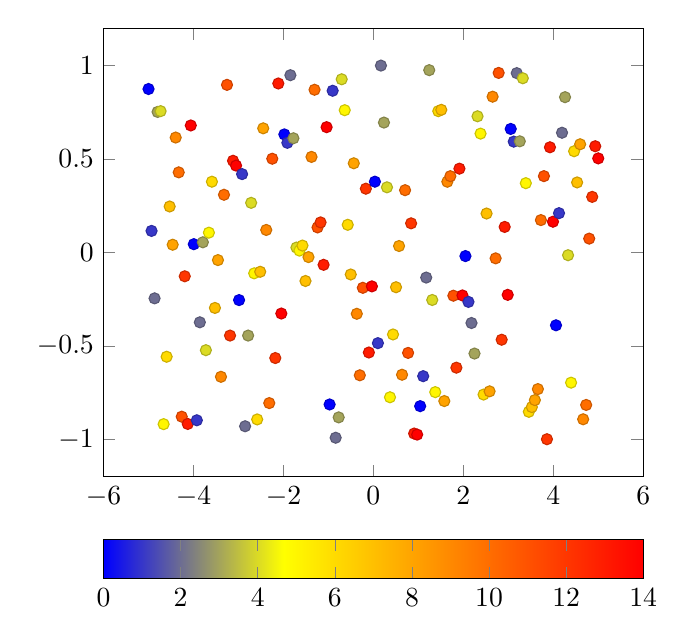
\begin{tikzpicture}
      \begin{axis}[colorbar horizontal]
        \addplot[only marks,scatter,
          scatter src={mod(\coordindex,15)},samples=150]
          {rand};
      \end{axis}
  \end{tikzpicture}}

\end{frame}

\begin{frame}[t]

  \frametitle{Search-Based Testing}
  \framesubtitle{Use a fitness function to guide the search to ``good'' values}

  \vspace*{.25in}
  \hspace{.25in}
  \resizebox{3.5in}{!}{
    \begin{tikzpicture}
      \begin{axis}[
          domain=0:1,
          xmax=1,
          ymax=1,
        ]
        \addplot3[surf] {x*y};
        \addplot3[solarizedRebase0,/pgfplots/quiver,
            quiver/u=y,
            quiver/v=x,
            quiver/w=0,
            quiver/scale arrows=0.1,
          -stealth,samples=10] {1};
      \end{axis}
  \end{tikzpicture}}

\end{frame}

\begin{frame}
  \frametitle{Performance of Search-based Software Testing}
   \tikzstyle{proc} = [draw, thick, fill=solarizedViolet, text centered, rounded corners,
    text=solarizedRebase02, draw=solarizedViolet]

\tikzstyle{prochighlight} = [draw, thick, fill=solarizedOrange, text centered, rounded corners,
    text=solarizedRebase02, draw=solarizedOrange]

\tikzstyle{procold} = [draw, thick, fill=solarizedViolet!75, text centered, rounded corners,
    text=solarizedRebase02, draw=solarizedViolet!75]

\tikzstyle{procchanged} = [draw, thick, fill=solarizedViolet!75, text centered, rounded corners,
    text=solarizedRebase02, draw=solarizedViolet!75]

\tikzstyle{prochighlightold} = [draw, thick, fill=solarizedOrange!75, text centered, rounded corners,
    text=solarizedRebase02, draw=solarizedOrange!75]

\tikzstyle{prochighlightchanged} = [draw, thick, fill=solarizedYellow!75, text centered, rounded corners,
    text=solarizedRebase02, draw=solarizedYellow!75]

\tikzstyle{proctest} = [draw, thick, fill=solarizedOrange, text centered, rounded corners,
text=solarizedBase02, draw=solarizedOrange]

\tikzstyle{procnew} = [draw, thick, fill=solarizedGreen, text centered, rounded corners,
    text=solarizedRebase02, draw=solarizedGreen]

\tikzstyle{procyellow} = [draw, thick, fill=solarizedYellow, text centered, rounded corners,
    text=solarizedRebase02, draw=solarizedYellow]

\tikzstyle{procred} = [draw, thick, fill=solarizedRed, text centered, rounded corners,
    text=solarizedRebase02, draw=solarizedRed]

\tikzstyle{io} = [ellipse, draw, thick, fill=solarizedBlue, draw=solarizedBlue, text=solarizedRebase02]

\tikzstyle{iopass} = [ellipse, draw, thick, fill=solarizedGreen, draw=solarizedGreen, text=solarizedRebase02]
\tikzstyle{iofail} = [ellipse, draw, thick, fill=solarizedRed, draw=solarizedRed, text=solarizedRebase02]
\tikzstyle{iohighlight} = [ellipse, draw, thick, fill=solarizedYellow, draw=solarizedYellow,
    text=solarizedRebase02]

\tikzstyle{iofailother} = [ellipse, draw, thick, fill=solarizedYellow, draw=solarizedYellow,
    text=solarizedRebase02]
\tikzstyle{wrongoutput} = [ellipse, draw, thick, fill=solarizedCyan, draw=solarizedCyan, text=solarizedRebase02]

\tikzstyle{special} = [draw, thick, fill=solarizedGreen, text centered, draw=solarizedGreen,
    text=solarizedBase02]
\tikzstyle{specialOrange} = [draw, thick, fill=solarizedOrange, text centered, draw=solarizedOrange,
    text=solarizedBase02]
\tikzstyle{specialGreen} = [draw, thick, fill=solarizedGreen, text centered, draw=solarizedGreen,
    text=solarizedBase02]
\tikzstyle{specialYellow} = [draw, thick, fill=solarizedYellow, text centered, draw=solarizedYellow,
    text=solarizedBase02]

\tikzstyle{pass} = [draw, thick, fill=solarizedGreen, text centered, draw=solarizedGreen, text=solarizedRebase02]
\tikzstyle{fail} = [draw, thick, fill=solarizedRed, text centered, draw=solarizedRed, text=solarizedRebase02]

\tikzstyle{feature} = [draw, thick, fill=solarizedOrange, text centered, text=solarizedRebase02, draw=solarizedOrange]

\tikzstyle{plain} = [draw, thick, fill=kapfhammerDarkGrey, text centered, text=solarizedRebase02, draw=kapfhammerDarkGrey]
\tikzstyle{featurecurve} = [draw, thick, fill=solarizedGreen, text centered, rounded corners]

   \def\scl{0.6}%scaling factor of the picture
\begin{tikzpicture}[
  scale=\scl,
  controlpanels/.style={yellow!30!brown!20!,rounded corners,draw=black,thick},
  screen/.style={green!50!black!60!,draw=black,thick},
  trace/.style={green!60!yellow!40!, ultra thick},
  smallbutton/.style={white,draw=black, thick},
  axes/.style={thick}]
  % \fill[green!30!blue!30!,rounded corners,draw=black,thick](0,0)
  %   rectangle (27.75,13.25);
  % \fill[fill=black!40!,draw=black,thick,rounded corners](0.25,0.25)
  %   rectangle (27.5,13.00);

% Lower right panel
  % \fill[controlpanels] (13.7,0.5) rectangle (27.1,6.2);
  % %Channels
  % % CH I
  % \draw[thick] (14.8,1.5) circle (0.7cm);
  % \fill[gray,draw=black,thick] (14.8,1.5) circle (0.5cm);
  % \fill[white,draw=black,thick] (14.8,1.5) circle (0.3cm);
  % \node[scale={1.5*\scl}] at (14.8,2.5) {CH I};
  % \draw[thick] (16.2,1.5) circle (0.4cm);
  % \fill[black!60!] (16.2,1.5) circle (0.3cm);
  % \draw[thick] (16.6,1.5) --(17,1.5)--(17,1.0);
  % \draw[thick] (16.7,1.0)--(17.3,1.0);
  % \draw[thick] (16.8,0.85)--(17.2,0.85);
  % \draw[thick] (16.9,0.70)--(17.1,0.70);
  % \draw[thick] (26.0,1.5) circle (0.7cm);
  % % CH II
  % \fill[gray,draw=black,thick] (26,1.5) circle (0.5cm);
  % \fill[white,draw=black,thick] (26,1.5) circle (0.3cm);
  % \node[scale={1.5*\scl}] at (26,2.5) {CH II};
  % \draw[thick] (24.6,1.5) circle (0.4cm);
  % \fill[black!60!] (24.6,1.5) circle (0.3cm);
  % \draw[thick] (24.2,1.5) --(23.7,1.5)--(23.7,1.0);
  % \draw[thick] (23.4,1.0)--(24.0,1.0);
  % \draw[thick] (23.5,0.85)--(23.9,0.85);
  % \draw[thick] (23.6,0.70)--(23.8,0.70);
  % \draw[thick] (26.0,1.5) circle (0.7cm);
  % Y-pos
  % \fill[smallbutton] (14.8,4.9) circle (0.3cm);
  % \node[scale={\scl}] at (14.8,5.5) {Y-pos I};
  % \fill[smallbutton] (26.0,4.9) circle (0.3cm);
  % \node[scale={\scl}] at (26.0,5.5) {Y-pos II};
  % Volt/div the foreach loop draws the two buttons
  \foreach \i / \b in {18/75,22.5/345}{
  %Second parameter of the loop is the angle of the index mark 
  \begin{scope}[xshift=\i cm,yshift=3.8cm,scale=0.85]
    \node[scale=\scl] at (0,2.3) {Volts/Div};
    \node[scale=\scl,black] at (-1,-2.4) {V};
    \node[scale=\scl,blue]  at (1,-2.4) {mV};
    \clip[rounded corners] (-2,-2) rectangle (2,2);
    \fill[black!30!,rounded corners,draw=black,thick] (-2,-2)
      rectangle (2,2);
    \fill[blue!50!black!20!,draw=black,thick]
      (30:1.1)--(30:3)--(3,-3)--(-90:3)--(-90:1.1) arc (-90:30:1.1);
    \draw[very thick,rounded corners](-2,-2) rectangle (2,2);
    \draw[thick] (0,0) circle (1.0);
    \foreach \i in {0,30,...,330}
      \draw[thick] (\i:1.2)--(\i:2.5);
    \foreach \i/\j in {15/50,45/.1,75/.2,105/.5,135/1,165/2,195/5,225/10,
      255/20,285/5,315/10,345/20} \node[scale=\scl,black] at (\i:1.7) {\j};
    \fill[blue!30!black!60!,draw=black,thick] (0,0) circle (0.8cm);
    % Here you set the right Volts/Div button
    \draw[ultra thick,red] (\b:0.3)--(\b:1.2);
  \end{scope}}
  \end{tikzpicture}

\end{frame}

\begin{frame}
    \frametitle{Search-based Software Testing}
    \HUGE O( )
\end{frame}




  %background
  \section{Background}

    \begin{frame}
      \frametitle{Doubling Experiment}
    \end{frame}

    \begin{frame}
      \frametitle{SchemaAnalyst}
      \begin{itemize}
        \item Criterion
        \item Data generator
        \item Schema
      \end{itemize}
    \end{frame}

    \section{Technique}
      \begin{frame}
        % \begin{figure}
          \frametitle{Method of Approach}
          \centering
          \tikzstyle{proc} = [draw, thick, fill=solarizedViolet, text centered, rounded corners,
    text=solarizedRebase02, draw=solarizedViolet]

\tikzstyle{prochighlight} = [draw, thick, fill=solarizedOrange, text centered, rounded corners,
    text=solarizedRebase02, draw=solarizedOrange]

\tikzstyle{procold} = [draw, thick, fill=solarizedViolet!75, text centered, rounded corners,
    text=solarizedRebase02, draw=solarizedViolet!75]

\tikzstyle{procchanged} = [draw, thick, fill=solarizedViolet!75, text centered, rounded corners,
    text=solarizedRebase02, draw=solarizedViolet!75]

\tikzstyle{prochighlightold} = [draw, thick, fill=solarizedOrange!75, text centered, rounded corners,
    text=solarizedRebase02, draw=solarizedOrange!75]

\tikzstyle{prochighlightchanged} = [draw, thick, fill=solarizedYellow!75, text centered, rounded corners,
    text=solarizedRebase02, draw=solarizedYellow!75]

\tikzstyle{proctest} = [draw, thick, fill=solarizedOrange, text centered, rounded corners,
text=solarizedBase02, draw=solarizedOrange]

\tikzstyle{procnew} = [draw, thick, fill=solarizedGreen, text centered, rounded corners,
    text=solarizedRebase02, draw=solarizedGreen]

\tikzstyle{procyellow} = [draw, thick, fill=solarizedYellow, text centered, rounded corners,
    text=solarizedRebase02, draw=solarizedYellow]

\tikzstyle{procred} = [draw, thick, fill=solarizedRed, text centered, rounded corners,
    text=solarizedRebase02, draw=solarizedRed]

\tikzstyle{io} = [ellipse, draw, thick, fill=solarizedBlue, draw=solarizedBlue, text=solarizedRebase02]

\tikzstyle{iopass} = [ellipse, draw, thick, fill=solarizedGreen, draw=solarizedGreen, text=solarizedRebase02]
\tikzstyle{iofail} = [ellipse, draw, thick, fill=solarizedRed, draw=solarizedRed, text=solarizedRebase02]
\tikzstyle{iohighlight} = [ellipse, draw, thick, fill=solarizedYellow, draw=solarizedYellow,
    text=solarizedRebase02]

\tikzstyle{iofailother} = [ellipse, draw, thick, fill=solarizedYellow, draw=solarizedYellow,
    text=solarizedRebase02]
\tikzstyle{wrongoutput} = [ellipse, draw, thick, fill=solarizedCyan, draw=solarizedCyan, text=solarizedRebase02]

\tikzstyle{special} = [draw, thick, fill=solarizedGreen, text centered, draw=solarizedGreen,
    text=solarizedBase02]
\tikzstyle{specialOrange} = [draw, thick, fill=solarizedOrange, text centered, draw=solarizedOrange,
    text=solarizedBase02]
\tikzstyle{specialGreen} = [draw, thick, fill=solarizedGreen, text centered, draw=solarizedGreen,
    text=solarizedBase02]
\tikzstyle{specialYellow} = [draw, thick, fill=solarizedYellow, text centered, draw=solarizedYellow,
    text=solarizedBase02]

\tikzstyle{pass} = [draw, thick, fill=solarizedGreen, text centered, draw=solarizedGreen, text=solarizedRebase02]
\tikzstyle{fail} = [draw, thick, fill=solarizedRed, text centered, draw=solarizedRed, text=solarizedRebase02]

\tikzstyle{feature} = [draw, thick, fill=solarizedOrange, text centered, text=solarizedRebase02, draw=solarizedOrange]

\tikzstyle{plain} = [draw, thick, fill=kapfhammerDarkGrey, text centered, text=solarizedRebase02, draw=kapfhammerDarkGrey]
\tikzstyle{featurecurve} = [draw, thick, fill=solarizedGreen, text centered, rounded corners]

          \newcommand{\mx}[1]{\mathbf{\bm{#1}}} % Matrix command
\newcommand{\vc}[1]{\mathbf{\bm{#1}}} % Vector command

% Define the layers to draw the diagram
\pgfdeclarelayer{background}
\pgfdeclarelayer{foreground}
\pgfsetlayers{background,main,foreground}

% Define distances for bordering
\def\blockdist{3.5}
\def\vertdist{2}

\hspace{-.25in}

\begin{minipage}{5in}

  \begin{center}

    \vspace*{-.3in}
    \begin{minipage}{4.5in}

      \begin{figure}

        \begin{center}

\begin{tikzpicture}[thick,scale=1, every node/.style={scale=1}]

  \path[use as bounding box] (-3.0,2.5) rectangle (10,-2);

    \path[->]<1-> node[proc, text width=15ex]
    (sa) at (1.5,.75) {\centering \textit{SchemaAnalyst} \\ Execution};

    \path[->]<2-> node[io, left of=sa, yshift=0.70in, xshift=-1.25in,text width=7ex]
    (cc) {\centering Coverage \\ Criterion} (cc) edge node {} (sa);

    \path[->]<3-> node[io, left of=sa, yshift=0.0in, xshift=-1.25in,text width=7ex]
    (dg) {\centering Data \\ Generator} (dg) edge node {} (sa);

    \path[->]<4-6> node[io, left of=sa, yshift=-0.70in, xshift=-1.25in,text width=7ex]
    (ds) {\centering Database \\ Schema} (ds) edge node {} (sa);

    \path[->]<5> node[io, right of=sa, yshift=0.0in, xshift=1.25in,text width=7ex]
    (ts) {\centering Test \\ Suite \\} (sa) edge node {} (ts);

    \path[->]<6-> node[io, right of=sa, yshift=0.0in, xshift=1.25in,text width=7ex]
    (ts) {\centering Runtime} (sa) edge node {} (ts);

    \path[->]<7-> node[proc, below of=sa, yshift=-0.3in, xshift=0.0in,text width=15ex]
    (sd) {\centering Schema Doubler} (sd) edge node {Provides Schema} (sa);

    \path[->]<7-> node[io, left of=sa, yshift=-0.70in, xshift=-1.25in,text width=7ex]
    (ds) {\centering Database \\ Schema} (ds) edge node {} (sd);

    \path[->]<8-> node[io, left of=sa, yshift=-1.40in, xshift=-1.25in,text width=7ex]
    (dc) {\centering Doubler \\ Choice} (dc) edge node {} (sd);

    \path[->]<9-> node[proc, right of=sd, yshift=0.0in, xshift=1.25in,text width=15ex]
    (ca) {\centering Convergence \\ Algorithm} (ca) edge node [below=.20in]{Continue?} (sd);

    \path[->]<9-> (ts) edge node {} (ca);


\end{tikzpicture}

\end{center}

\end{figure}

\end{minipage}

\end{center}

\end{minipage}

        % \end{figure}
      \end{frame}

      \begin{frame}
        \frametitle{Doubling Database Schemas}
        \centering
        \tikzstyle{proc} = [draw, thick, fill=solarizedViolet, text centered, rounded corners,
    text=solarizedRebase02, draw=solarizedViolet]

\tikzstyle{prochighlight} = [draw, thick, fill=solarizedOrange, text centered, rounded corners,
    text=solarizedRebase02, draw=solarizedOrange]

\tikzstyle{procold} = [draw, thick, fill=solarizedViolet!75, text centered, rounded corners,
    text=solarizedRebase02, draw=solarizedViolet!75]

\tikzstyle{procchanged} = [draw, thick, fill=solarizedViolet!75, text centered, rounded corners,
    text=solarizedRebase02, draw=solarizedViolet!75]

\tikzstyle{prochighlightold} = [draw, thick, fill=solarizedOrange!75, text centered, rounded corners,
    text=solarizedRebase02, draw=solarizedOrange!75]

\tikzstyle{prochighlightchanged} = [draw, thick, fill=solarizedYellow!75, text centered, rounded corners,
    text=solarizedRebase02, draw=solarizedYellow!75]

\tikzstyle{proctest} = [draw, thick, fill=solarizedOrange, text centered, rounded corners,
text=solarizedBase02, draw=solarizedOrange]

\tikzstyle{procnew} = [draw, thick, fill=solarizedGreen, text centered, rounded corners,
    text=solarizedRebase02, draw=solarizedGreen]

\tikzstyle{procyellow} = [draw, thick, fill=solarizedYellow, text centered, rounded corners,
    text=solarizedRebase02, draw=solarizedYellow]

\tikzstyle{procred} = [draw, thick, fill=solarizedRed, text centered, rounded corners,
    text=solarizedRebase02, draw=solarizedRed]

\tikzstyle{io} = [ellipse, draw, thick, fill=solarizedBlue, draw=solarizedBlue, text=solarizedRebase02]

\tikzstyle{iopass} = [ellipse, draw, thick, fill=solarizedGreen, draw=solarizedGreen, text=solarizedRebase02]
\tikzstyle{iofail} = [ellipse, draw, thick, fill=solarizedRed, draw=solarizedRed, text=solarizedRebase02]
\tikzstyle{iohighlight} = [ellipse, draw, thick, fill=solarizedYellow, draw=solarizedYellow,
    text=solarizedRebase02]

\tikzstyle{iofailother} = [ellipse, draw, thick, fill=solarizedYellow, draw=solarizedYellow,
    text=solarizedRebase02]
\tikzstyle{wrongoutput} = [ellipse, draw, thick, fill=solarizedCyan, draw=solarizedCyan, text=solarizedRebase02]

\tikzstyle{special} = [draw, thick, fill=solarizedGreen, text centered, draw=solarizedGreen,
    text=solarizedBase02]
\tikzstyle{specialOrange} = [draw, thick, fill=solarizedOrange, text centered, draw=solarizedOrange,
    text=solarizedBase02]
\tikzstyle{specialGreen} = [draw, thick, fill=solarizedGreen, text centered, draw=solarizedGreen,
    text=solarizedBase02]
\tikzstyle{specialYellow} = [draw, thick, fill=solarizedYellow, text centered, draw=solarizedYellow,
    text=solarizedBase02]

\tikzstyle{pass} = [draw, thick, fill=solarizedGreen, text centered, draw=solarizedGreen, text=solarizedRebase02]
\tikzstyle{fail} = [draw, thick, fill=solarizedRed, text centered, draw=solarizedRed, text=solarizedRebase02]

\tikzstyle{feature} = [draw, thick, fill=solarizedOrange, text centered, text=solarizedRebase02, draw=solarizedOrange]

\tikzstyle{plain} = [draw, thick, fill=kapfhammerDarkGrey, text centered, text=solarizedRebase02, draw=kapfhammerDarkGrey]
\tikzstyle{featurecurve} = [draw, thick, fill=solarizedGreen, text centered, rounded corners]

        \pgfdeclarelayer{background}
\pgfdeclarelayer{foreground}
\pgfsetlayers{background,main,foreground}

\begin{minipage}{.5in}

\begin{center}

\begin{minipage}{.45in}

\begin{figure}

\begin{center}

\begin{tikzpicture}[thick,scale=1, every node/.style={scale=1}]

\path[use as bounding box] (-5.0,2.5) rectangle (10,-2);

\node<1-> (table) [proc] {
    \begin{tabular}{l}
    \textbf{Table}\\ \hline
        \parbox{4cm}{
            \begin{itemize}
                \color{solarizedBase02}
                \item Column 1
                \item Column 2
                \item \dots
                \item Column n
            \end{itemize}
        }
    \end{tabular}
};

\path<2-> (table.west)+(-2,0) node (nn1) [proctest] {NOT NULL};
\path<2-> [draw, ->] (nn1.east) -- node [above] {} (table.179);

\path[->]<3-> node[proctest, right of=table, yshift=0.0in,xshift=1.25in, minimum width=7ex] (pkey) {PRIMARY KEY} (pkey.west) edge node {} (table.340);

\path[->]<4-> node[proctest, above of=nn1, yshift=0.0in, xshift=0.0in, minimum width=7ex] (unique) {UNIQUE} (unique.east) edge node {} (table);


\path[->]<5-> node[proctest, below of=pkey, yshift=0.0in, xshift=0.0in, minimum width=7ex] (check) {CHECK} (check.west) edge node {} (table);

\path[->]<6-> node[proctest, above of=pkey, yshift=0.0in, xshift=0.0in, minimum width=7ex] (fkey) {FORIEGN KEY} (fkey.west) edge node {} (table);

\path[->]<6-> node[proc, above of=fkey, yshift=0.0in, xshift=1.5in,
minimum width=7ex] (rtab) {} (rtab) edge node {} (fkey.east);



\path<7-> (nn1.south)+(0,-.5) node (nn2) [proctest] {NOT NULL};
\path<7-> [draw, ->] (nn2.east) -- node [above] {} (table.181);

\end{tikzpicture}

\end{center}
\end{figure}
\end{minipage}
\end{center}
\end{minipage}

      \end{frame}

    \section{Experiment Design}
      \begin{frame}
        \frametitle{Experiments}
        \begin{columns}
        \column{0.5\textwidth}
        \begin{itemize}
          \item Parameters Studied
          \item Cluster
        \end{itemize}
          \column{0.5\textwidth}
          \begin{figure}
            \includegraphics[width=\textwidth]{iceberg2014.jpg}
          \end{figure}
      \end{columns}
      \end{frame}

    \section{Results}
      \begin{frame}
        \frametitle{Results}
        \begin{itemize}
          \item BigOh Table
          \item Data mining
          \item Statistical Tests
        \end{itemize}
      \end{frame}

      \begin{frame}
        \frametitle{Criterion}
        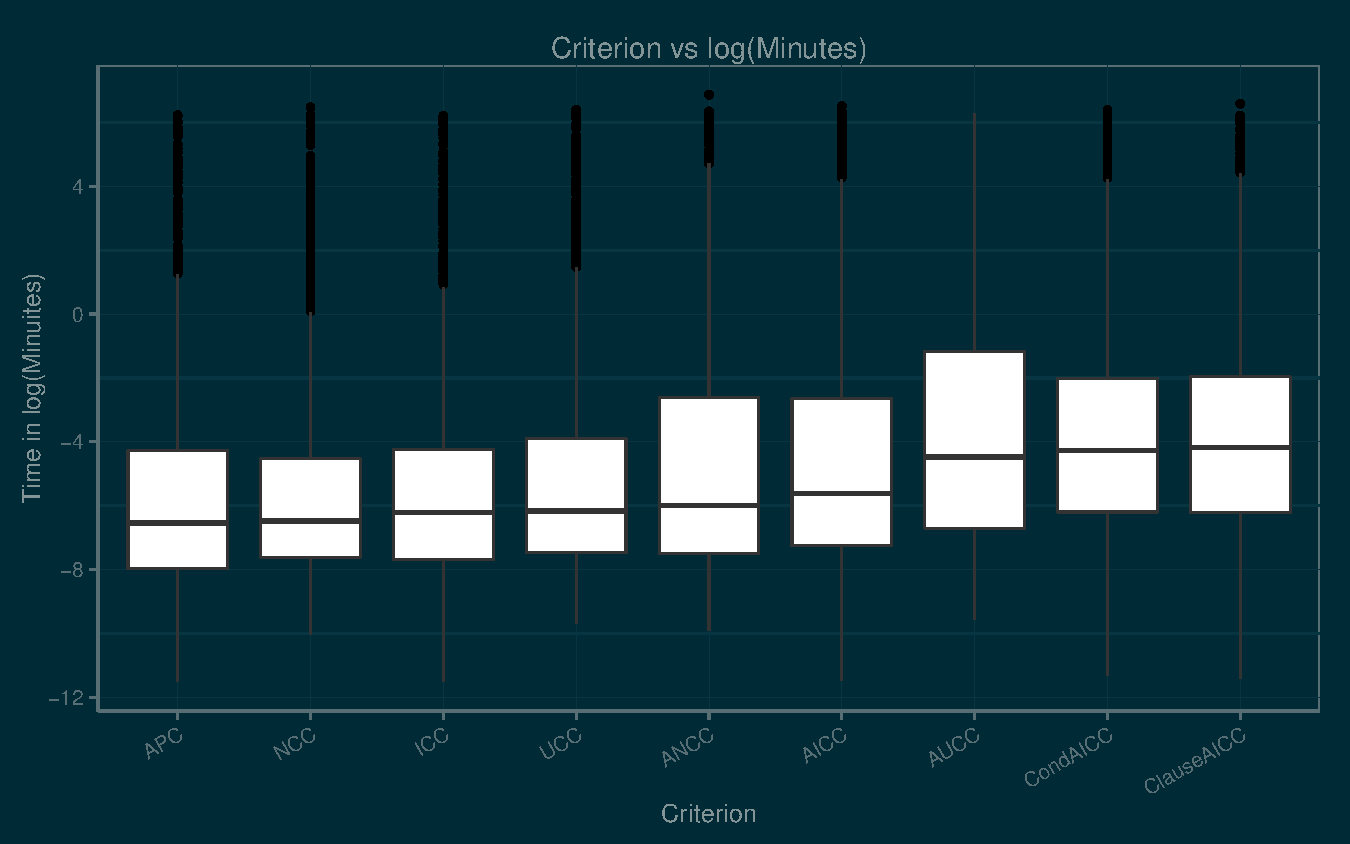
\includegraphics[width=\textwidth]{CriterionBox}
      \end{frame}

      \begin{frame}
        \frametitle{Data Generator}
        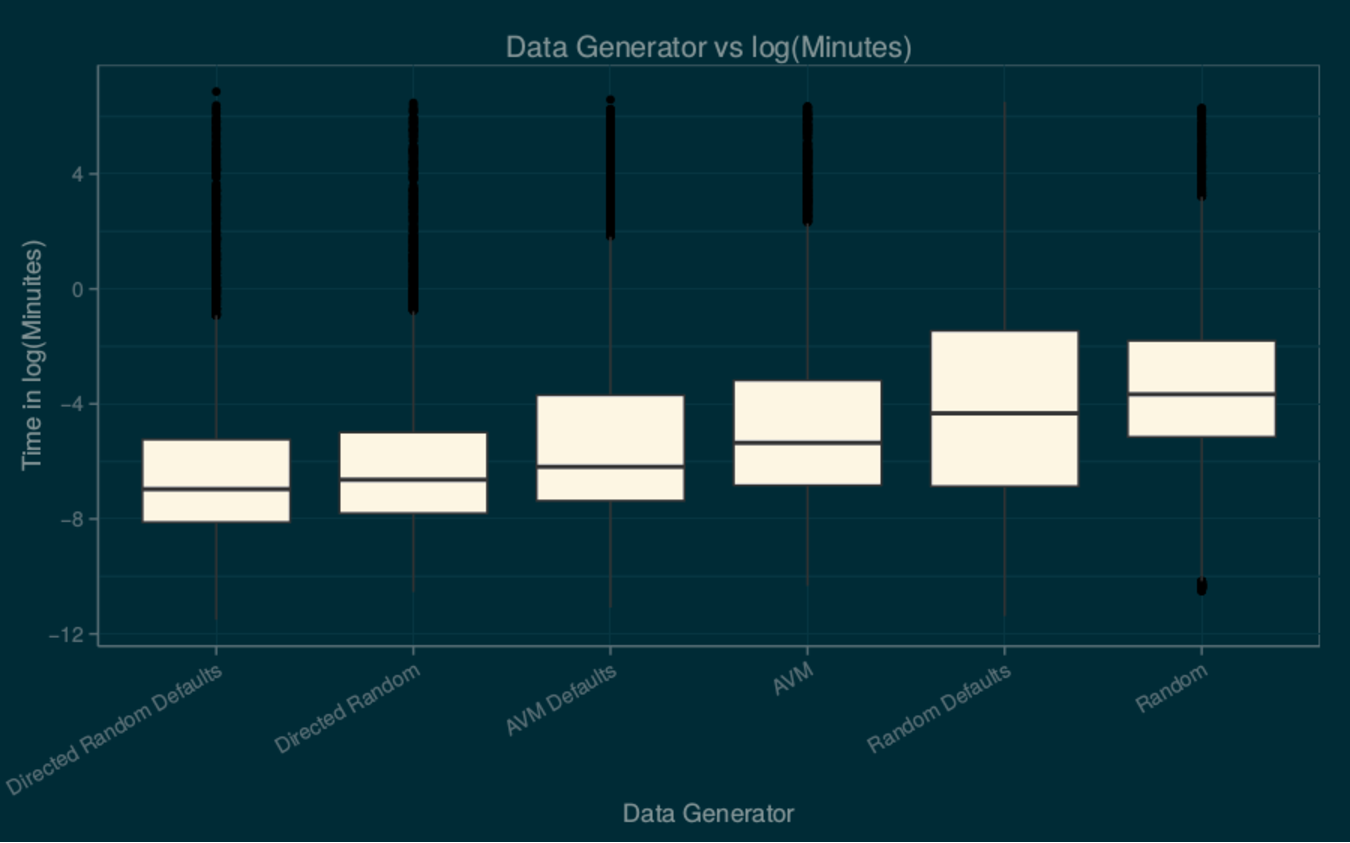
\includegraphics[width=\textwidth]{DataGeneratorBox}
      \end{frame}


    \section{Conclusion}
      \begin{frame}
        \frametitle{Conclusion}
      \end{frame}

      % \begin{frame}
      %   \titlepage
      % \end{frame}

      \end{document}
